El objetivo de esta sección será volver a experimentar, ahora que ya superamos una etapa de ajuste para las heurísticas, sobre un nuevo conjunto de instancias. También analizaremos las heurísticas y metaheurísticas en un caso cuya solución exacta conocemos de antemano. Finalmente, sacaremos en limpio algunas conclusiones sobre lo que fue la segunda parte de este trabajo, que consistió en probar diversas heurísticas. 

\subsection{Parámetros que elegimos}
Vamos a comparar la búsqueda local contra la búsqueda tabú. Para eso escogimos las configuraciones que nos resultaron más satisfactorias:
\begin{itemize}
	\item Para la búsqueda local escogimos INTERCAMBIAR, que mostraba tener una relación calidad-tiempo razonable.
	\item Para \emph{tabu search} escogimos el criterio de parada que espera a que hayan 500 iteraciones sin mejorar. En cuanto al tamaño de la lista tabú, en la medida que no había grandes diferencias, escogimos 200. Si bien con 20 era marginalmente más rápido y la calidad era la misma, pareciera que la mejora no es tanta como para sacrificar la robustez que puede brindar el tener una lista significativamente más larga.
\end{itemize}

Nuevamente, la comparación contra el algoritmo goloso se encuentra implícita pues tomamos las diferencias de aristas y tiempos con respecto a esta heurística.

\subsection{Resultados}
A continuación pasamos a presentar los resultados obtenidos para esta experimentación. A diferencia de otros experimentos como acá no hizo falta realizar muchas iteraciones de experimentación para ajustar cosas, se pudo tomar una muestra más significativa de instancias.

En las figuras de la \ref{fig:7-calidad1} a la \ref{fig:7-calidad3} se puede apreciar algo bastante esperable: \emph{tabu search} devuelve significativamente más aristas tanto en promedio como, más notoriamente, en los máximos. Sin embargo, algo muy destacable que no se aprecia directamente en los gráficos es que hubo algunos casos dónde la búsqueda local mejoró la solución golosa y la búsqueda tabú no. Esto es consistente con el hecho de que aunque sea una metaheurística de búsqueda global sigue sin tener garantías reales de encontrar un óptimo verdadero. Sin embargo, en los casos en los que esto ocurre la diferencia no es muy superior a una o dos aristas; mientras que en los casos que \emph{tabu search} es superior se pueden llegar a apreciar diferencias bastante más significativas.

Algo que fue transversal a toda la experimentación desde la sección 5 hasta aquí, aunque no fue mencionado antes, es que en general hay más casos donde los refinamientos no pudieron mejorar la solución que en los que sí se pudo. Además, en los casos en los que sí se mejoró generalmente la cantidad de aristas extras era poco significativa con respecto a la cantidad aristas que encontraba inicialmente el goloso\footnote{De hecho esta es quizás la razón más fuerte por la que graficamos diferencias y no los valores en crudo, pues notar la superioridad de un algoritmo u otro hubiese resultado complicado. También el hecho de que hayan muchos casos donde la diferencia es 0 produce que en general los gráficos de calidad que vimos tengan en genral barras bastante bajas con varianzas muy altas.}. Estos no son detalles menores pues nos hablan de que la calidad de las soluciones provistas por la heurística golosa es generalmente bastante alta \emph{per se}, o bien que simplemente son difíciles de mejorar. Un dato a tener en cuenta.
 
\begin{figure}[H]
\centering
\begin{minipage}{0.49\textwidth}
  \centering
    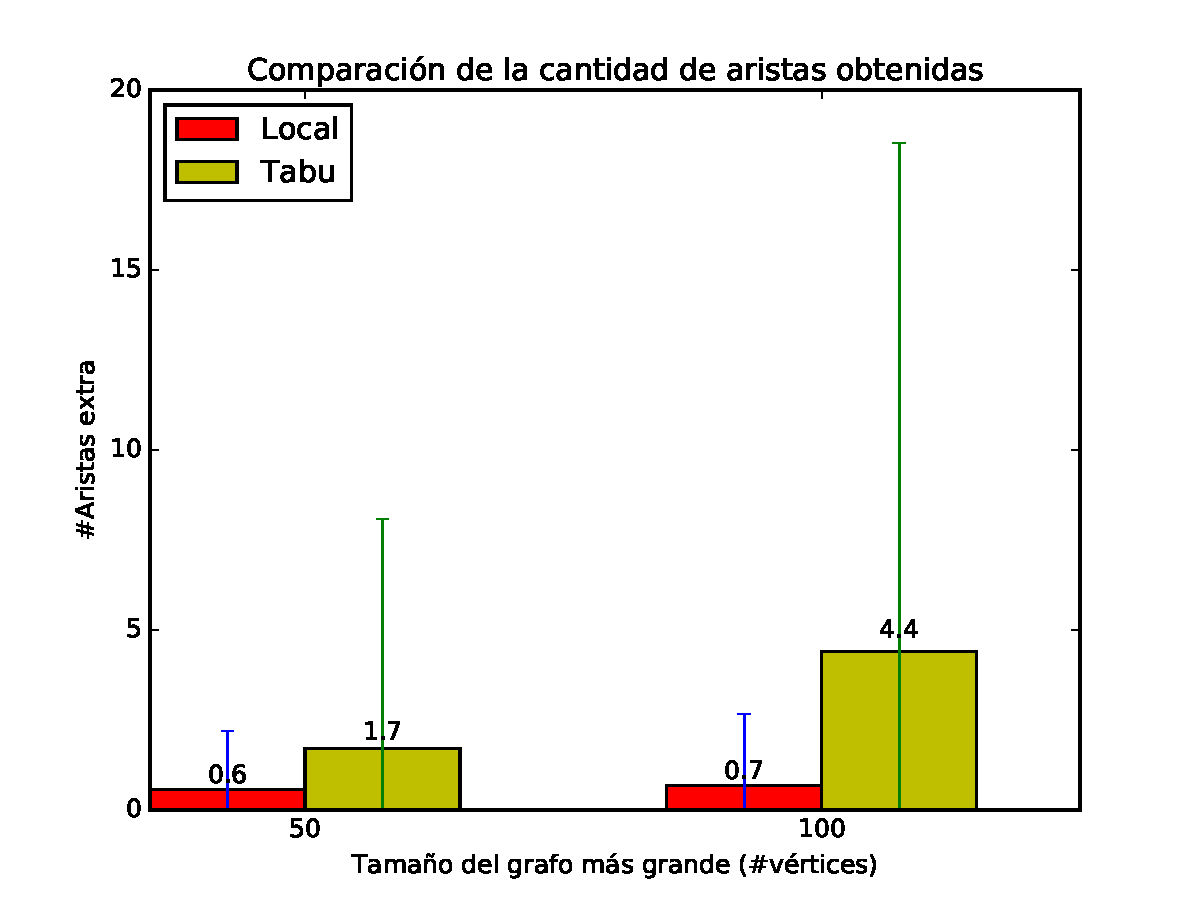
\includegraphics[width=1\textwidth]{graficos/problema_7/calidad0.pdf}
  \caption{}
  \label{fig:7-calidad1}
\end{minipage}%
\hspace{0.01\textwidth}
\begin{minipage}{0.49\textwidth}   
  \centering
    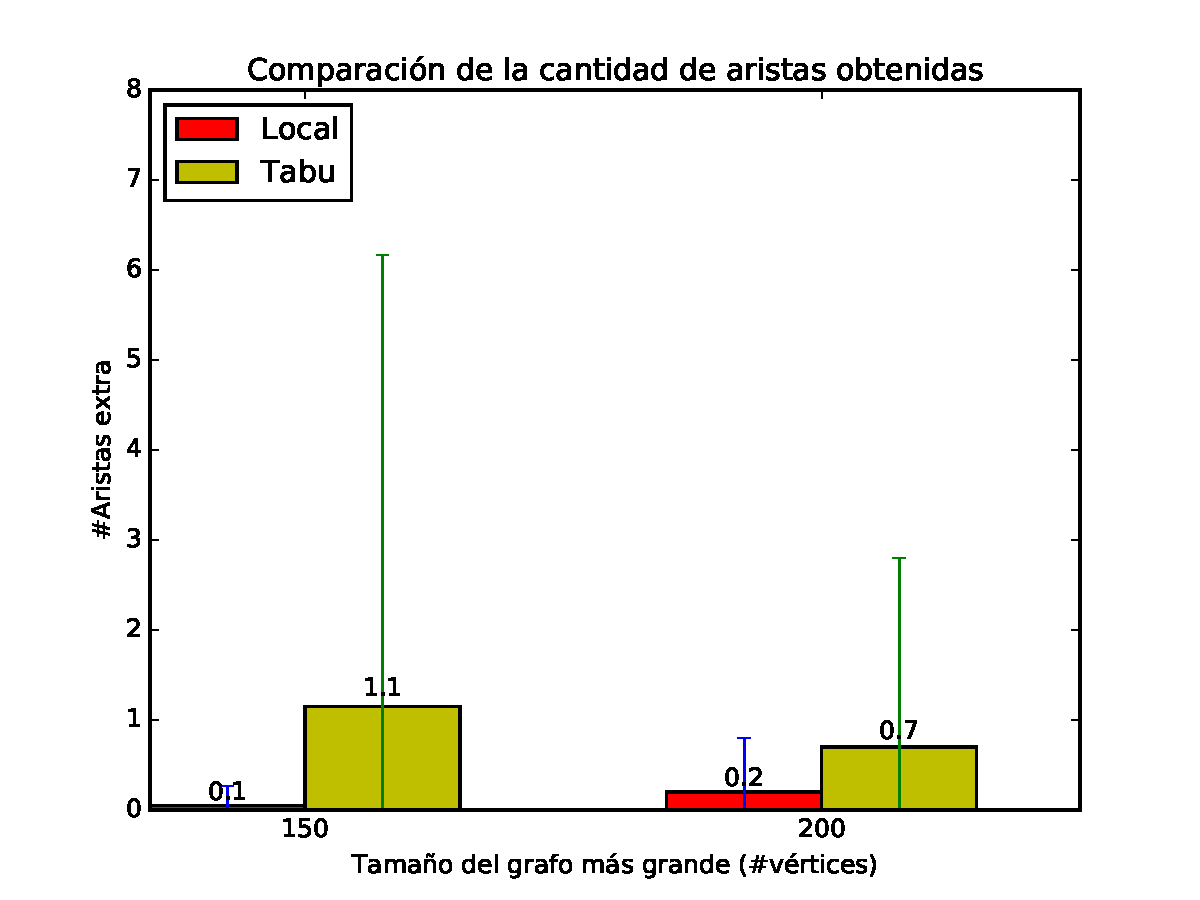
\includegraphics[width=1\textwidth]{graficos/problema_7/calidad2.pdf} 
  \caption{}
  \label{fig:7-calidad2}
\end{minipage}

\begin{minipage}{0.49\textwidth}
  \centering
    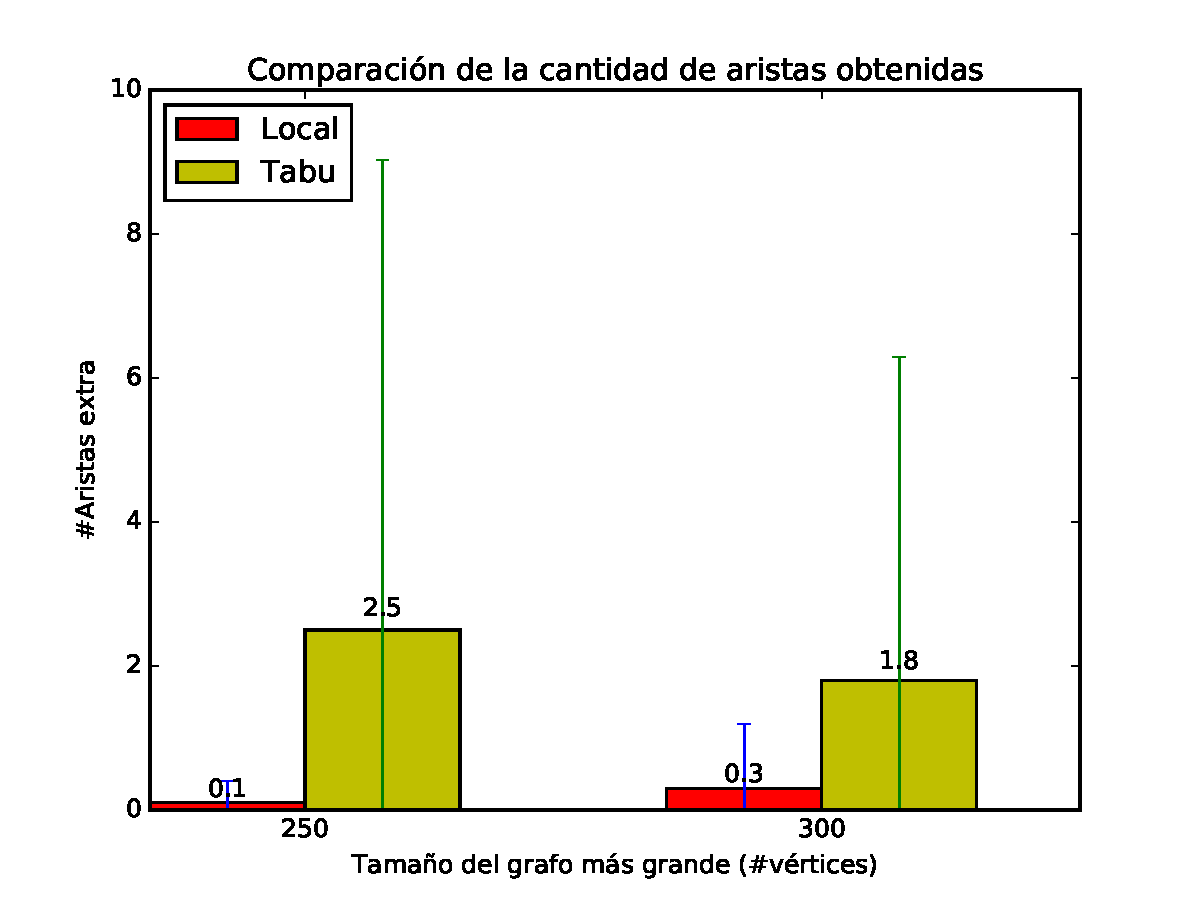
\includegraphics[width=1\textwidth]{graficos/problema_7/calidad4.pdf}
  \caption{}
  \label{fig:7-calidad3}
\end{minipage}%
\end{figure}

En las figuras de la \ref{fig:7-tiempo1} a la \ref{fig:7-tiempo3} se comparan los tiempos de ejecución. La diferencia es abrumadora en favor de la búsqueda local. No hay mucho más para decir al respecto pues en definitiva era esperable, aunque sí resulta sorprendente una diferencia tan abultada. 

Finalmente en las figuras \ref{fig:7-cociente1} a \ref{fig:7-cociente3} vemos los gráficos para la relación calidad/tiempo. Resulta claro al ver esot que dicha relación está dominada por el tiempo más que por la calidad (algo parecida ocurría en la sección 5, aunque aquí resulta más evidente). Un detalle a destacar es que aunque en general siempre usamos segundos como medida del tiempo, en este caso concreto tuvimos que usar minutos de forma que fuese apreciable el valor para la metaheurística.

\begin{figure}[H]
\centering
\begin{minipage}{0.49\textwidth}
  \centering
    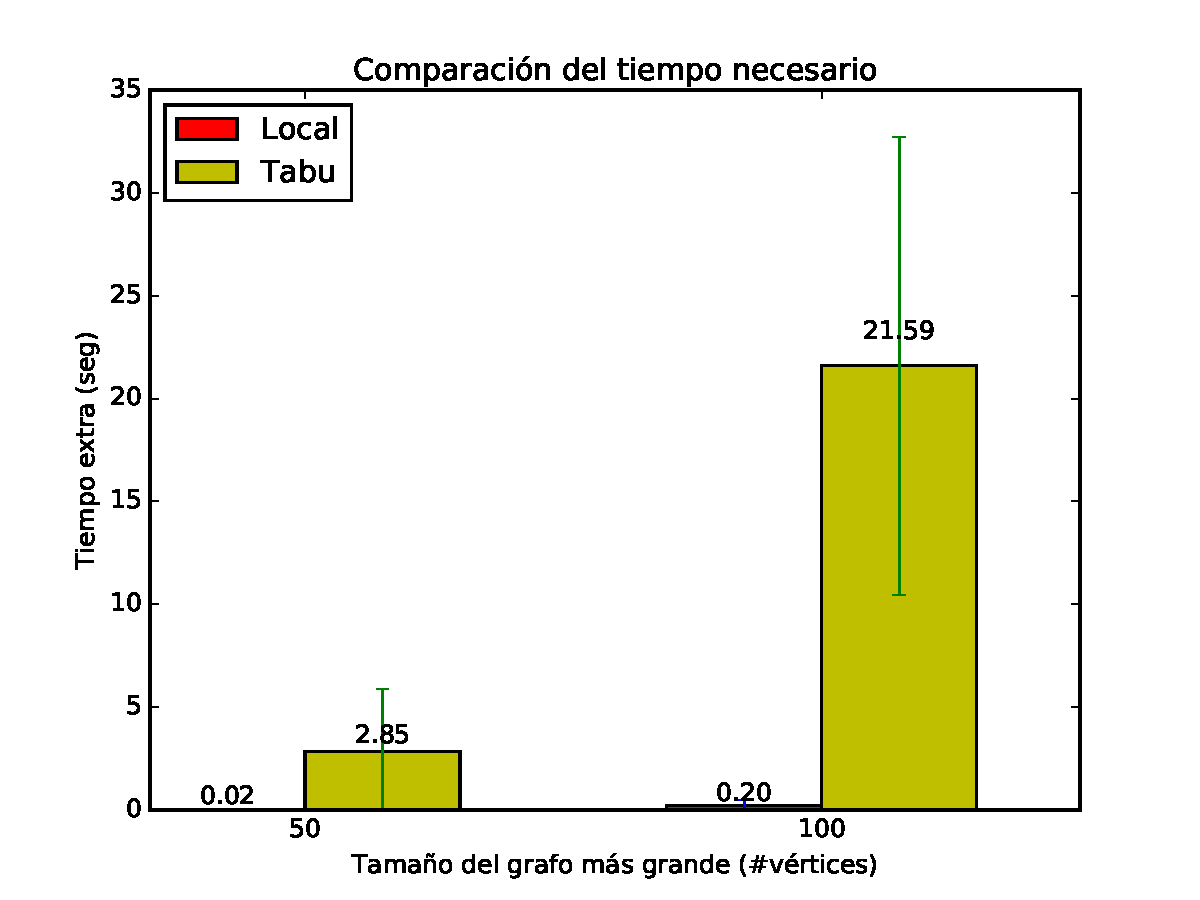
\includegraphics[width=1\textwidth]{graficos/problema_7/tiempo0.pdf}
  \caption{}
  \label{fig:7-tiempo1}
\end{minipage}%
\hspace{0.01\textwidth}
\begin{minipage}{0.49\textwidth}   
  \centering
    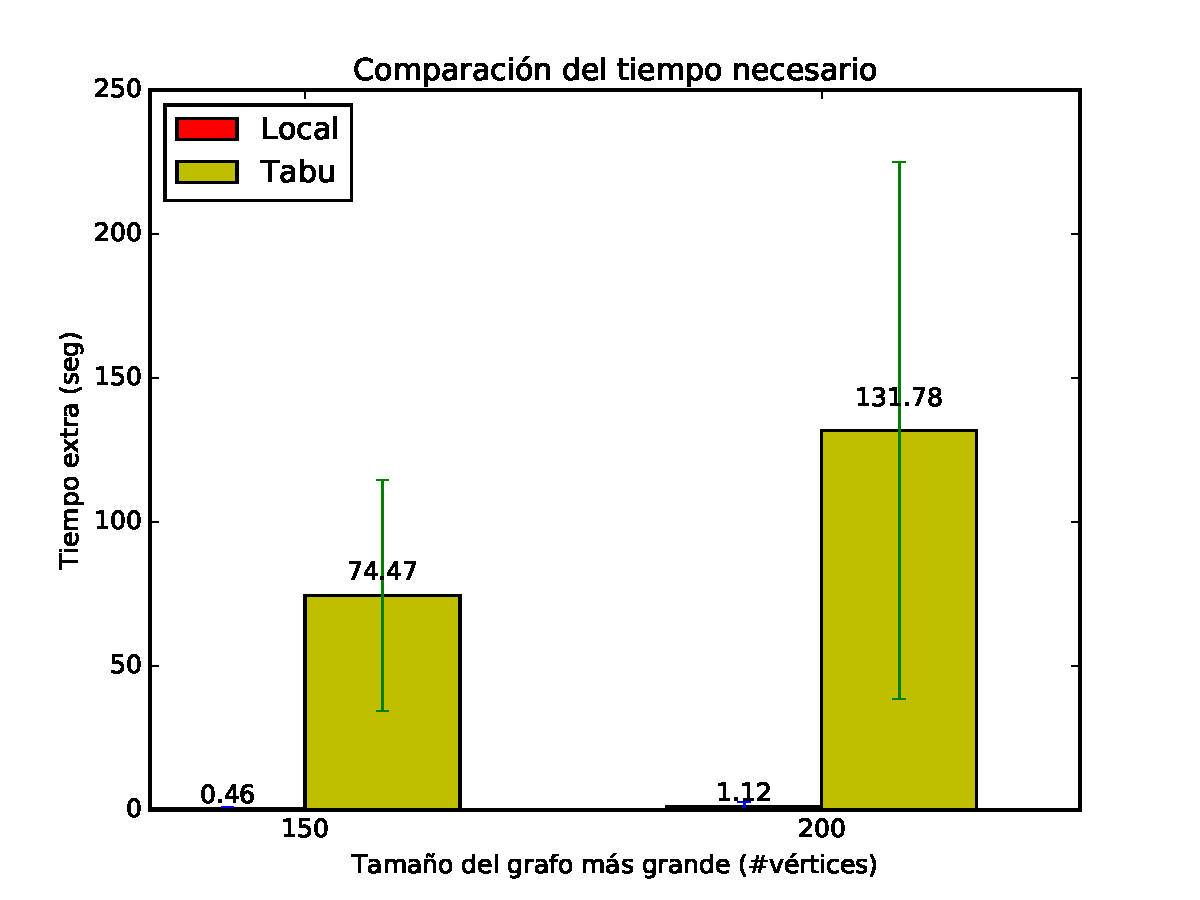
\includegraphics[width=1\textwidth]{graficos/problema_7/tiempo2.pdf} 
  \caption{}
  \label{fig:7-tiempo2}
\end{minipage}

\begin{minipage}{0.49\textwidth}
  \centering
    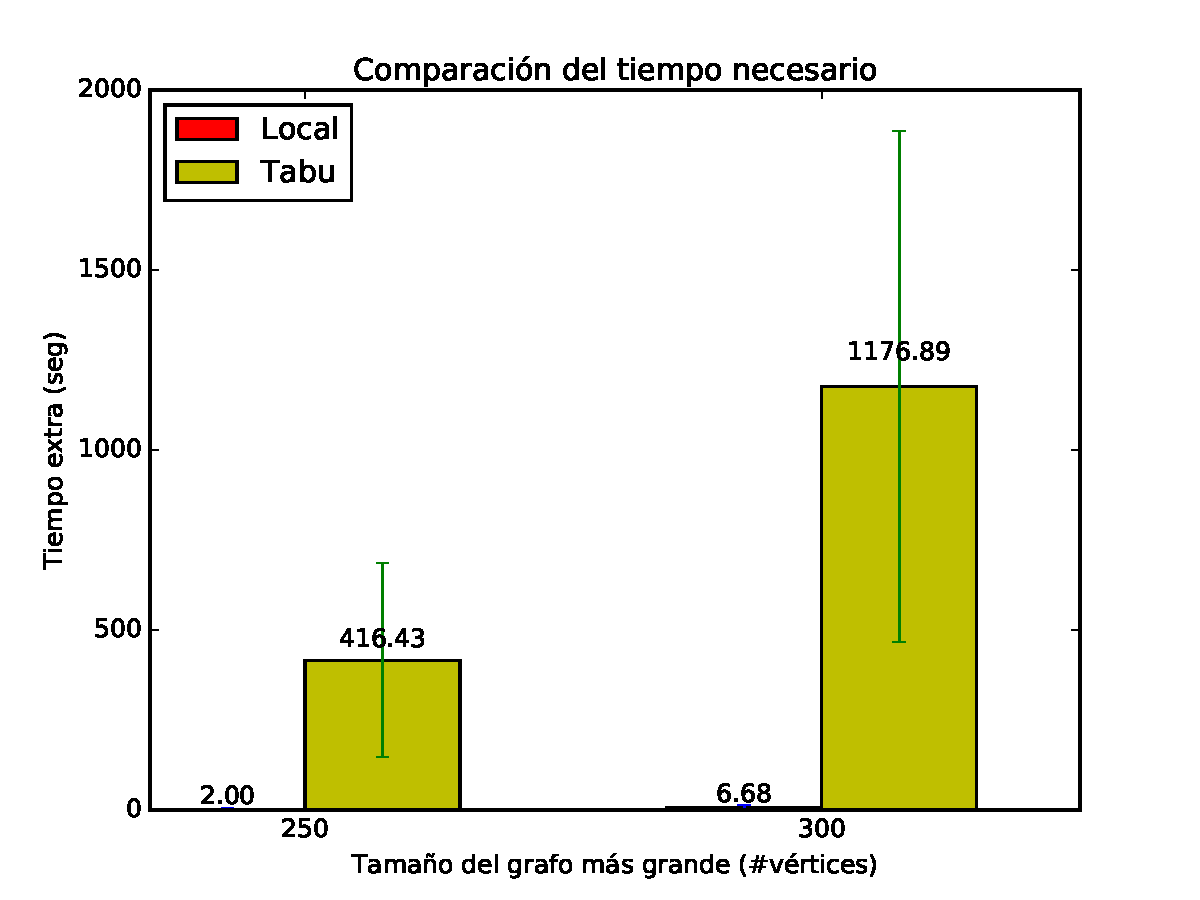
\includegraphics[width=1\textwidth]{graficos/problema_7/tiempo4.pdf}
  \caption{}
  \label{fig:7-tiempo3}
\end{minipage}%
\end{figure}

\begin{figure}[H]
\centering
\begin{minipage}{0.49\textwidth}
  \centering
    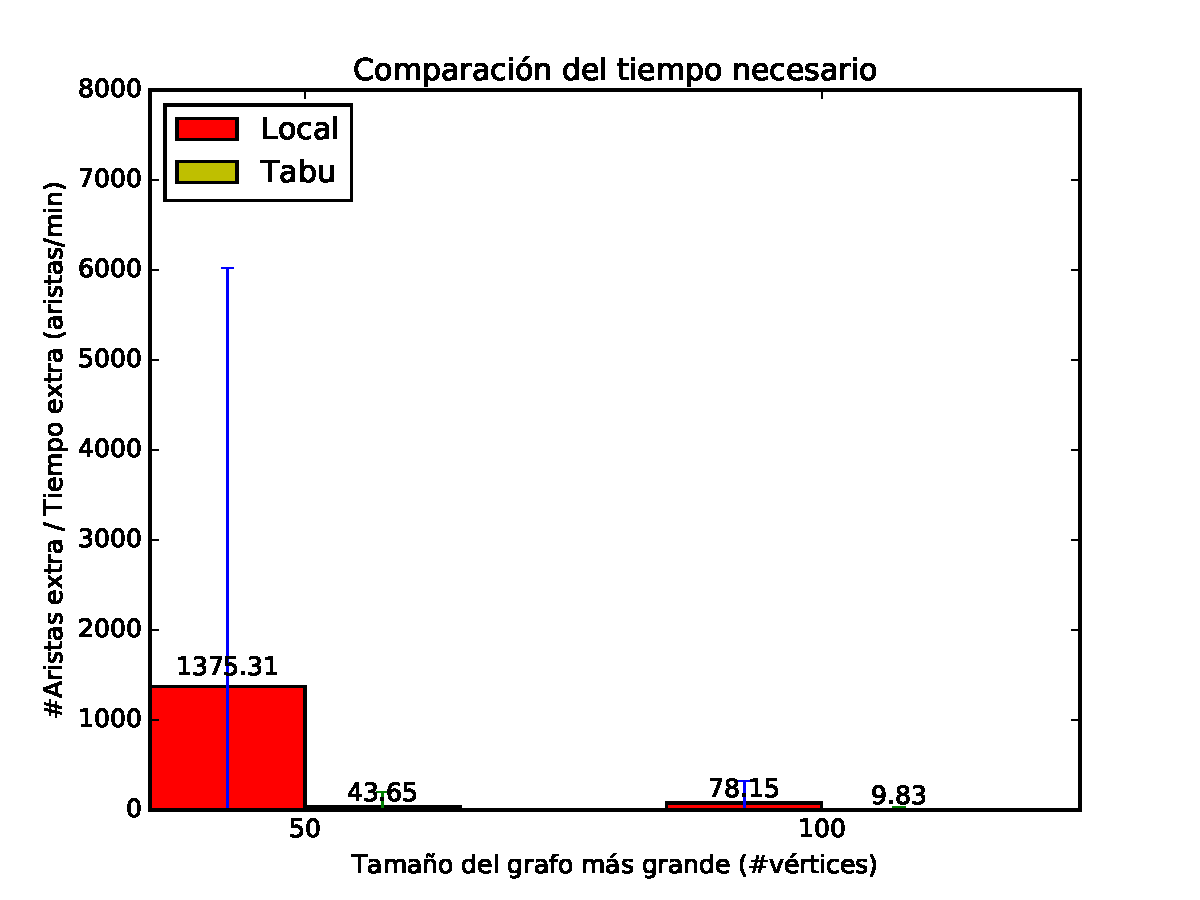
\includegraphics[width=1\textwidth]{graficos/problema_7/cociente0.pdf}
  \caption{}
  \label{fig:7-cociente1}
\end{minipage}%
\hspace{0.01\textwidth}
\begin{minipage}{0.49\textwidth}   
  \centering
    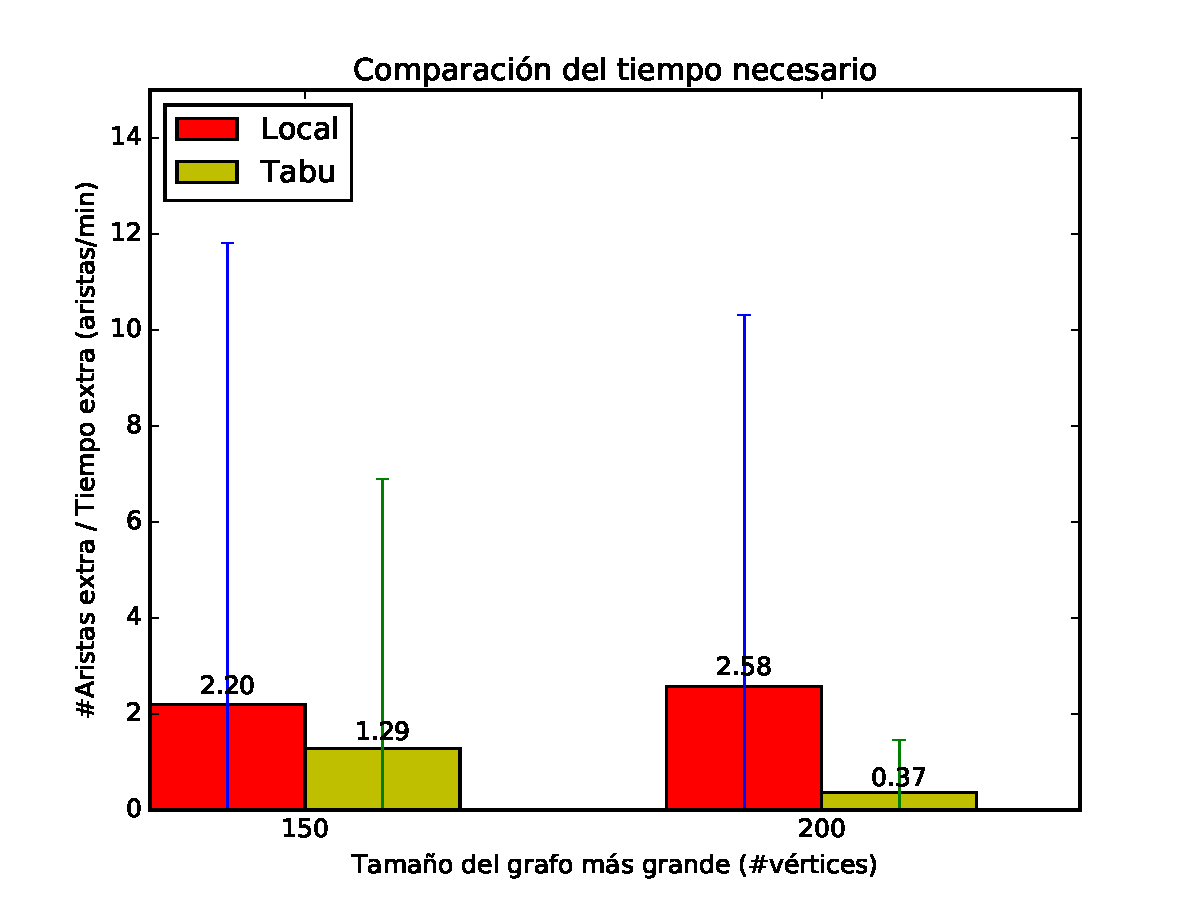
\includegraphics[width=1\textwidth]{graficos/problema_7/cociente2.pdf} 
  \caption{}
  \label{fig:7-cociente2}
\end{minipage}

\begin{minipage}{0.49\textwidth}
  \centering
    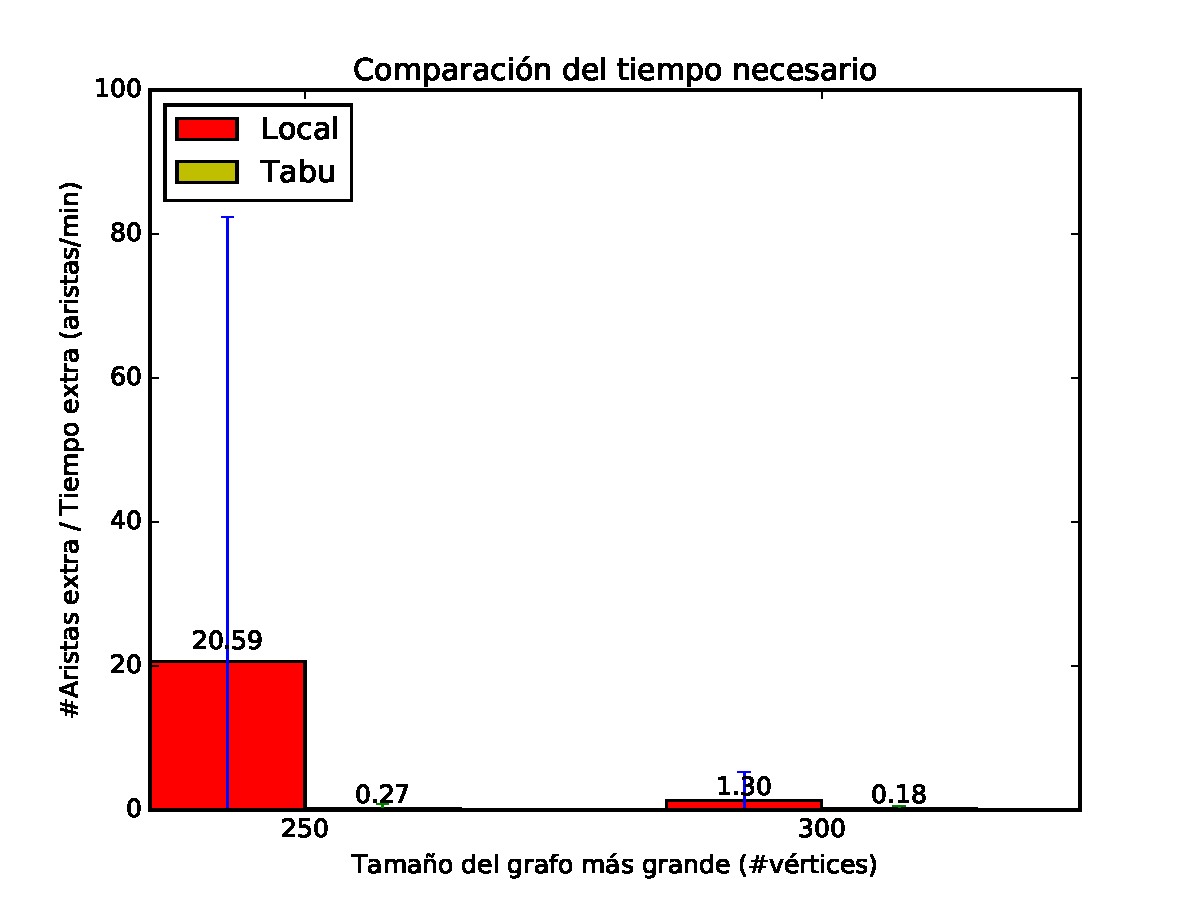
\includegraphics[width=1\textwidth]{graficos/problema_7/cociente4.pdf}
  \caption{}
  \label{fig:7-cociente3}
\end{minipage}%
\end{figure}

\subsection{Comparación con el algoritmo exacto}

Algo interesante que podemos preguntarnos es cómo se comparan nuestros algoritmos con el algoritmo exacto.

Sin embargo, como vimos anteriormente, el algoritmo exacto es extremadamente lento, por lo que un experimento ``clásico'', en el que se generan casos al azar y se corren los algoritmos sobre ellos no es viable.

Por esta razón, decidimos elegir una familia de grafos para la cual conozcamos de antemano, por sus características, la solución exacta, sin necesidad de correr el algoritmo exacto. 

Esta familia es precisamente la familia que encontramos como ``contraejemplo'' en el ejercicio del algoritmo goloso. Era la familia que nos permitía demostrar que el algoritmo no es $\alpha$-aproximado para ningún $\alpha > 0$. 

Recordemos los grafos y analicemos sus propiedades.


\begin{tikzpicture}[shorten >=1pt,auto,node distance=1.9cm,
                    semithick]
  \tikzstyle{every state}=[fill=red,draw=none,text=white]

	\node[state]	(0)		 		  {$2$};
	\node[state]	(1) [right of=0]  {$4$};
	\node[state]	(2) [below of=0]  {$3$};
	\node[state]	(3) [left of=0] 	  {$0$};
	\node[state]	(4) [above of=0]	  {$1$};
	\node[state]	(5) [right of=1]	  {$5$};
	\node[state]	(6) [above of=5]  {$6$};
	\node[state]	(7) [right of=6]  {$7$};
	\node[state]	(8) [right of=5]  {$8$};
	\node[state, fill=blue]	(9) [right of=8]	  {$0$};
	\node[state, fill=blue]	(10) [above of=9]  {$1$};
	\node[state, fill=blue]	(11) [right of=9]  {$2$};
	\node[state, fill=blue]	(12) [right of=10]  {$3$};


	\path	
		(0) edge[]				node {} (1)
         	edge[]				node {} (2)
         	edge[]				node {} (4)
         	edge[]				node {} (3)
		(1) edge[]				node {} (5)
		(5) edge[]				node {} (6)
		    edge[]				node {} (7)
		    edge[]				node {} (8)
		(6) edge[]				node {} (7)
		    edge[]				node {} (8)
		(7) edge[]				node {} (8)
		(9) edge[]				node {} (10)
		    edge[]				node {} (11)
		    edge[]				node {} (12)
		(10) edge[]				node {} (11)
		    edge[]				node {} (12)
		(11) edge[]				node {} (12);

\end{tikzpicture}

En nuestro caso utilizaremos una pequeña variación de este grafo (la única diferencia es que la arista que une a la estrella con el completo no sale de un brazo, si no de el centro de la estrella).

Como vimos anteriormente, el algoritmo goloso devuelve una solución muy mala siempre, dado que mapea al grafo completo azul con el grafo estrella rojo. 

Otra cosa que puede observarse es que, por como son nuestras heurísticas de búsqueda local, esa solución (la del goloso) es un mínimo local para todas estas soluciones. Esto puede chequearse muy fácilmente viendo la forma de los grafos y las soluciones (cualquier vecino a la solución del goloso es igual o peor que la solución del goloso).

Sin embargo, el tabú search viene a solucionar este problema, debido a la función de aspiración, que nos permite saltar a una solución aunque sea peor que la que tenemos, si todas lo son.

Enunciadas nuestras hipótesis sobre la experimentación, veamos los resultados.

\begin{figure}[H]
 \centering
	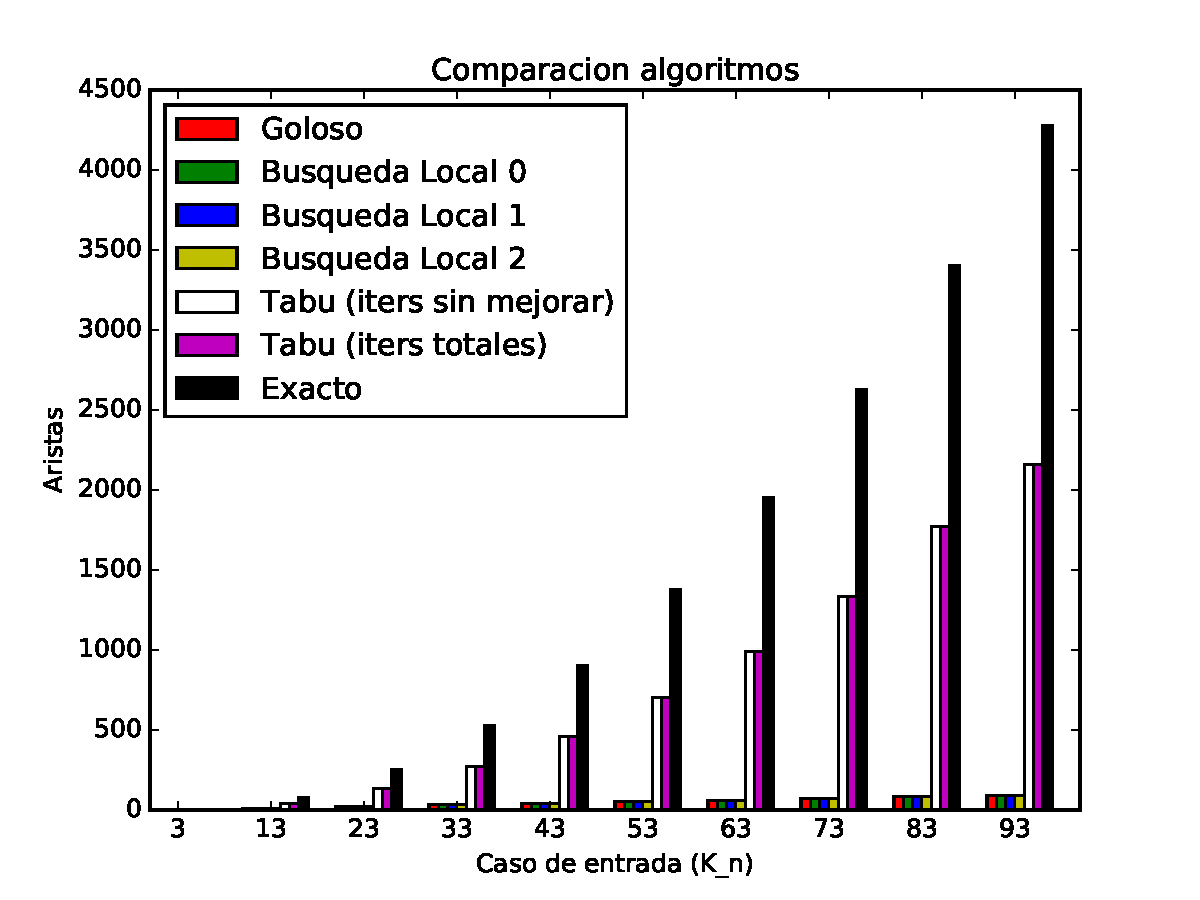
\includegraphics[width=0.9\textwidth]{graficos/problema_7/exacto0.pdf}
	\caption{}
	\label{fig:problema7-exacto0}
\end{figure}


Puede verse que sucede lo que esperábamos. Es decir, la solución del algoritmo goloso es muy mala, y la de las búsquedas locales no lo mejora.

Sin embargo, el tabú search permite mejorar mucho las soluciones. De todos modos, al igual que antes, no se observan diferencias notorias entre los dos criterios de parada del algoritmo: el secreto del éxito reside en las buenas vecindades que elegimos.

\subsection{Conclusiones}
Como cierre para las últimas tres secciones donde experimentamos y discutimos ampliamente sobre distintas heurísticas y metaheurísticas, pasamos en limpio algunas conclusiones.

Encontramos que la solución golosa para casos generales no resulta tan mala como se esperaba inicialmente. Incluso analizamos otra variante golosa mucho más rudimentaria en la que simplemente se mapeaban los nodos de mayor grado de cada grafo, y sorpresivamente no tuvo tan malos resultados. Sin embargo, como el otro era consistentemente mejor en calidad lo preferimos por sobre el más simple, aunque también fuese significativamente más rápido. 

Entre las búsqueda locales vimos que en muchos casos permitían mejorar la solución golosa, aunque en general nunca demasiado. Para obtener soluciones que sacarán levemente mayor diferencia teníamos que recurrir a una vecindad, que aunque se podía recorrer polinomialmente, en la práctica el costo a pagar era muy alto. 

Como propuesta superadora probamos distintas implementaciones de la metaheurística de búsqueda local \emph{tabu search} variando sus parámetros más clásicos. Lo que obtuvimos fue un resultado muy satisfactorio desde el punto de vista de la calidad, aunque nuevamente pagando un fuerte precio en tiempo. También vimos en esta sección que sigue estando lejos de ser un algoritmo exacto.

En definitiva, a la hora de escoger una u otra alternativa habrá que considerar fuertemente el contexto de uso: en un ámbito científico como el planteado por el problema posiblemente sea preferible recurrir a la búsqueda tabú aunque pueda requerir horas o días para obtener el resultado deseado, pues seguramente la situación resulte lo suficientemente delicada como para requerir la mejor solución posible. También es la mejor alternativa en general para instancias relativamente chicas. En contextos menos críticos donde se prefiera la velocidad, INTERCAMBIAR, REMPLAZAR o incluso la misma heurística golosa resultan alternativas más sensatas.  


